\documentclass[]{article}
\usepackage{authblk}
\usepackage{tikz}
\usepackage{graphics}
\usepackage{graphicx}
\usepackage{pst-node,pst-plot}
\usepackage{svg}


%opening
\title{Practical implementation for fair exchange of two pieces of information using a single Bitcoin transaction involving punishment for non-cooperating party}
\author{Shahpour Moavenat}
\affil{Lykke Corp}

\begin{document}

\maketitle

\begin{abstract}
There are some conditions in which it is required to exchange two pieces of information between parties who do not trust each other; two of these conditions are mentioned in the next section. This problem has been vastly studied, for example in \cite{ray2002} and \cite{asokan99}. In this article a method is presented so that by building and publishing a custom built bitcoin transaction, each party should either reveal the agreed upon piece of information or if after some designated time passed, pay an agreed upon sum of bitcoin to the other party.


\end{abstract}

\section{Introduction}
Two samples of the problems of interest are: a- Assuming two parties have sent two different assets to each other through a configuration of lightning network \cite{lightning} and the assets have arrived locked by a pre-image (R). If now parties exchange the pre-images, actually they can exchange their assets\footnote{This could be also somehow achieved by a method known as atomic swapping \cite{lnswap}, the author does not think the name is appropriate since the operation is actually divisible to smaller pieces, also the control of the operation resides in hands of one party, so it may require more analysis.}. b- Assume two parties want to exchange their signatures for example (RSA signatures on a document), the desired final state is that either each party should have the other one's signature or neither should have the other's one (zkSNARK \cite{ethzkSNARK} could be used as a method to make sure what is provided is actually the signature). In the case of requirement for strong fairness (which roughly means at end of exchange either both parties have the required information or no party has any additional information about the other party item), this problems is proved not to be solvable in peer-to-peer configuration without a trusted third party \cite{impossible}.

In the proposed protocol in this article, instead of relying on a third party which is required to be trusted, we use Bitcoin blockchain capabilities to ensure the desired exchange operation will happen or otherwise the non cooperating party will be punished by an agreed upon sum.

\textbf{Related work:} A similar high level study is available including some suggestions to introduce some changes to Bitcoin protocol in \cite{andrychowicz}. In \cite{maxwell2016} a method using zkSNARKs\cite{ethzkSNARK} to pay for a solution to a problem is described. The current article uses the idea described there.

\section{Bitcoin transaction with penalty}
Using Bitcoin network, we can ask each party to put a collateral in a Bitcoin transaction that will be returned to him/her when (s)he contributes the secret publicly, otherwise after some timeout the collateral will be spendable by the other party. By using this method each party is forced to release the secret or pay a penalty, if (s)he does not do so.

The transaction should be of segregated witness \cite{segwit} type, so its transaction id could be known without signatures and monitored on blockchain, when a party who signs the transaction the second, if did not broadcast the transaction (which may have lower probability, since before this signature exchange phase, both parties have followed some other procedures and somehow showed their intentions for exchange; although more analysis may be required here), the transaction could be monitored for further actions.

So the built transaction will have two inputs and two outputs, two inputs are the collaterals each party puts in to the contract so that it could be punished if the release of desired information is not done in the desired time frame.

\subsection{Transaction details}

The desired transaction will have 2 inputs, and two outputs, as in Figure \ref{fig:transaction}.

\begin{figure}[h!]
	\centering
	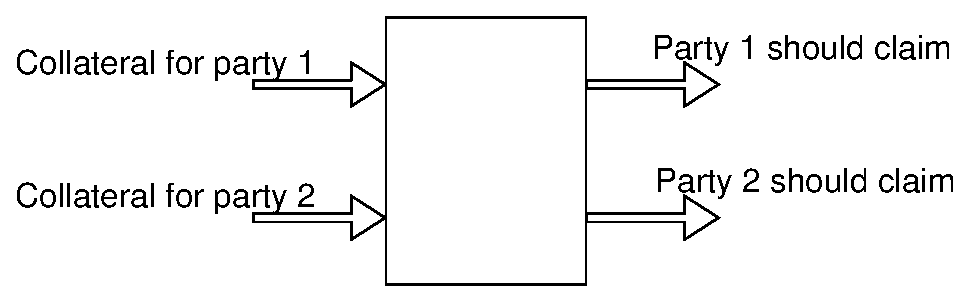
\includegraphics[width=1\textwidth]{images/transaction.eps}
	\caption{Segwit transaction	to be signed and posted to blockchain}
	\label{fig:transaction}
\end{figure}

Input amounts are what each party needs to put into transaction (contract) as collateral, that if the corresponding output was not claimed, will become available to the other party after sometime as a mechanism of punishment for not following the protocol. If the output is claimed, this will release the information required for the exchange.

Output script will generally be like following (Actual details will depend on the hash type):

\begin{verbatim}
OP_SHA256
<Hash of pre-image> OP_EQUAL
OP_IF
<Self Pubkey>
OP_ELSE
<block_height+number of blocks in timeout period> OP_CHECKLOCKTIMEVERIFY OP_DROP
<Other party Pubkey>
OP_ENDIF
OP_CHECKSIG
\end{verbatim}

The above output could be claimed by the party putting collateral, if it releases the pre-image of the hash. Otherwise after some designated time, the other party could claim the collateral as punishment for not releasing the pre-image. So if every party is interested in claiming its collateral (which normally should be case), the result would be release of pre-images to blockchain which means every party would become aware of the other party's pre-image and exchange of pre-images has happened.

\section{Extension}

Some information to be exchanged may need some checks that may not be as simple and applicable to output script as a simple hash calculation described above. For example, we can consider exchange of two digital signatures for a hash. In this case the required checks will include the following: if the signature is correct and actually belongs to the expected public key. Including all the checks in the output script may create some problems, including being it possible or not and also large number of instructions (which for example in Ethereum network will lead to large amount of ethers used for calculation, and in Bitcoin will lead to high transaction fees).

One possible workaround would be sending an encrypted version of the signature to the other party and also the hash of the encryption key for the signature. Then there would be a proof which justifies, by possession of actual encryption key (for which the hash is available), the receiving party could decrypt the encrypted signature which is also the desired one for the preknown public key. These kind of proofs could be provided by zkSNARKs\cite{ethzkSNARK}. Then what would actually be exchanged over blockchain are those pre-images for the hashed encryption keys.

This method could be probably applied to large set of exchange problems.

\section{Other considerations}

The proposed protocol over Bitcoin has one advantage, it is symmetrical. Which means after the transaction is posted over blockchain no party has the upper hand over the other, this is because in Bitcoin we can have transactions which can have multiple inputs. In some other blockchains, it will become a matter of interest of who does what and when (The order becomes important).

Related to the above is one problem of the protocol that is about what would happen if the party signing the transaction as second will not broadcast the transaction? A possible benefit for the cheating party to do this, would be to broadcast the transaction when it is not expected and after timeout claim the collateral. One solution would be to monitor blockchain for a specific time, and if the transaction was not brodcasted, the collateral input will be spent (which would cost a fee), so the unbroadcasted transaction could no more be broadcasted. To achieve this goal the transaction id to be monitored should be independent of signatures using approaches like segregated witness\cite{segwit}.

To partially cover the above scenario, in order to reduce the risk of possible cheating party to gain a position in which (s)he can cheat, a method would be to select the party who signs the transaction first by random. A method for this would to run a game as follows: Each party provides the other one a random number between 0 and 9, and if the sum was even the first (pre-agreed) party will provide the initial signature otherwise the second party will do so; thus the selection of the party who provides the first signature becomes random. Providing the random number would like following; each party will provide to the other one the proof of execution of a function (zkSNARK) that takes the a-encrypted number, b-hash of encryption key and c- encryption key as the inputs (the last one being a private input) and verifies that that the encryption key hashes to the provided hash, and the encrypted number decrypts to a number between 0 and 9. After proofs were verified the encryption keys are exchanged and each party will know the sum of numbers is even or odd, thus the protocol initiator is randomly chosen and the cheating party will probably not continue if (s)he is chosen to provide the signature first.

Another possible implementation problem would be high transaction fees, be it the exchange transaction itself or the protection mechanism described above. One method to overcome this problem would be to use similar blockchains or Bitcoin forks supporting required operations, like multiple input transactions and segregated witness.

\section{Conclusion}

In this article I have presented a method to exchange two pieces of information using Bitcoin blockchain, and if one party is not keeping it words, (s)he will be punished by paying a fine. Future path to be solved is the reduction of amount of fees paid and also a better solution to a little asymetrical phase described in previous section.

\begin{thebibliography}{9}
	\bibitem{ray2002}
	Indrajit Ray, Indrakshi Ray, 
	\textit{Fair Exchange in E-commerce},
	ACM SIGecom Exchanges, Volume 3 Issue 2, Spring, 2002,
	pp 9-17. 
	
	\bibitem{asokan99}
	    N. Asokan,Victor Shoup,Michael Waidner,
	    \textit{Optimistic fair exchange of digital signatures},
	    revised and extended version of Eurocrypt 99 Abstract and of IBM research report RZ 2973, 1999. Available from http://www.shoup.net/papers/fex.pdf
		
	\bibitem{maxwell2016}
	Gregory Maxwell,
	\textit{The first successful Zero-Knowledge Contingent Payment}, 2016.
	Available from https://bitcoincore.org/en/2016/02/26/zero-knowledge-contingent-payments-announcement/
	
	\bibitem{ethzkSNARK}
	Christian Reitwiessner,
	\textit{zkSNARKs in a nutshell}, 2016.
	Available from
	https://blog.ethereum.org/2016/12/05/zksnarks-in-a-nutshell/
	
	\bibitem{lnswap}
	Conner Fromknecht,
	\textit{Connecting Blockchains: Instant Cross-Chain Transactions On Lightning},
	Available from https://blog.lightning.engineering/announcement/2017/11/16/ln-swap.html
	
	\bibitem{andrychowicz}
	Marcin Andrychowicz, Stefan Dziembowski, Daniel Malinowski, Lukasz Mazurek,
	\textit{Fair Two-Party Computations via Bitcoin Deposits}, Financial Cryptography and Data Security: FC 2014 Workshops, BITCOIN and WAHC 2014, Christ Church, Barbados, March 7, 2014, Revised Selected Papers, pp 105-121.
	
	\bibitem{segwit}
	Eric Lombrozo, Johnson Lau, Pieter Wuille,
	\textit{Segregated Witness Bitcoin Improvement Proposal},
	Available from https://github.com/bitcoin/bips/blob/master/bip-0141.mediawiki
	
	\bibitem{impossible}
	H. Pagnia, F. C. Gärtner, 
	\textit{On the impossibility of fair exchange without a trusted
	third party}, Technical report, 1999.

	\bibitem{lightning}
	Joseph Poon, Thaddeus Dryja,
	\textit{The Bitcoin Lightning Network: Scalable Off-Chain Instant Payments}, DRAFT Version 0.5.9.2, 2016.
	    
\end{thebibliography}
\end{document}
